\section{Value Function}
\begin{frame}{}
    \LARGE Reinforcement Learning: \textbf{Value Function}
\end{frame}

\begin{frame}{Value Function}
\begin{itemize}
    \item How good is a state?
    \pause
    \item The \textbf{value function} at state s, is the expected cumulative reward from following the policy from state s:
    $$V^{\pi}(s) = \mathbb{E} \left [ \sum_{t \geq 0} \gamma^t r_t | s_0=0, \pi \right ]$$
    \item Computing the value function is generally impractical, but we can try
to approximate (learn) it
    \item The benefit is credit assignment: see directly how an action affects
future returns rather than wait for rollouts

\end{itemize}

\end{frame}

\begin{frame}{Value Function}
\begin{figure}
\centering
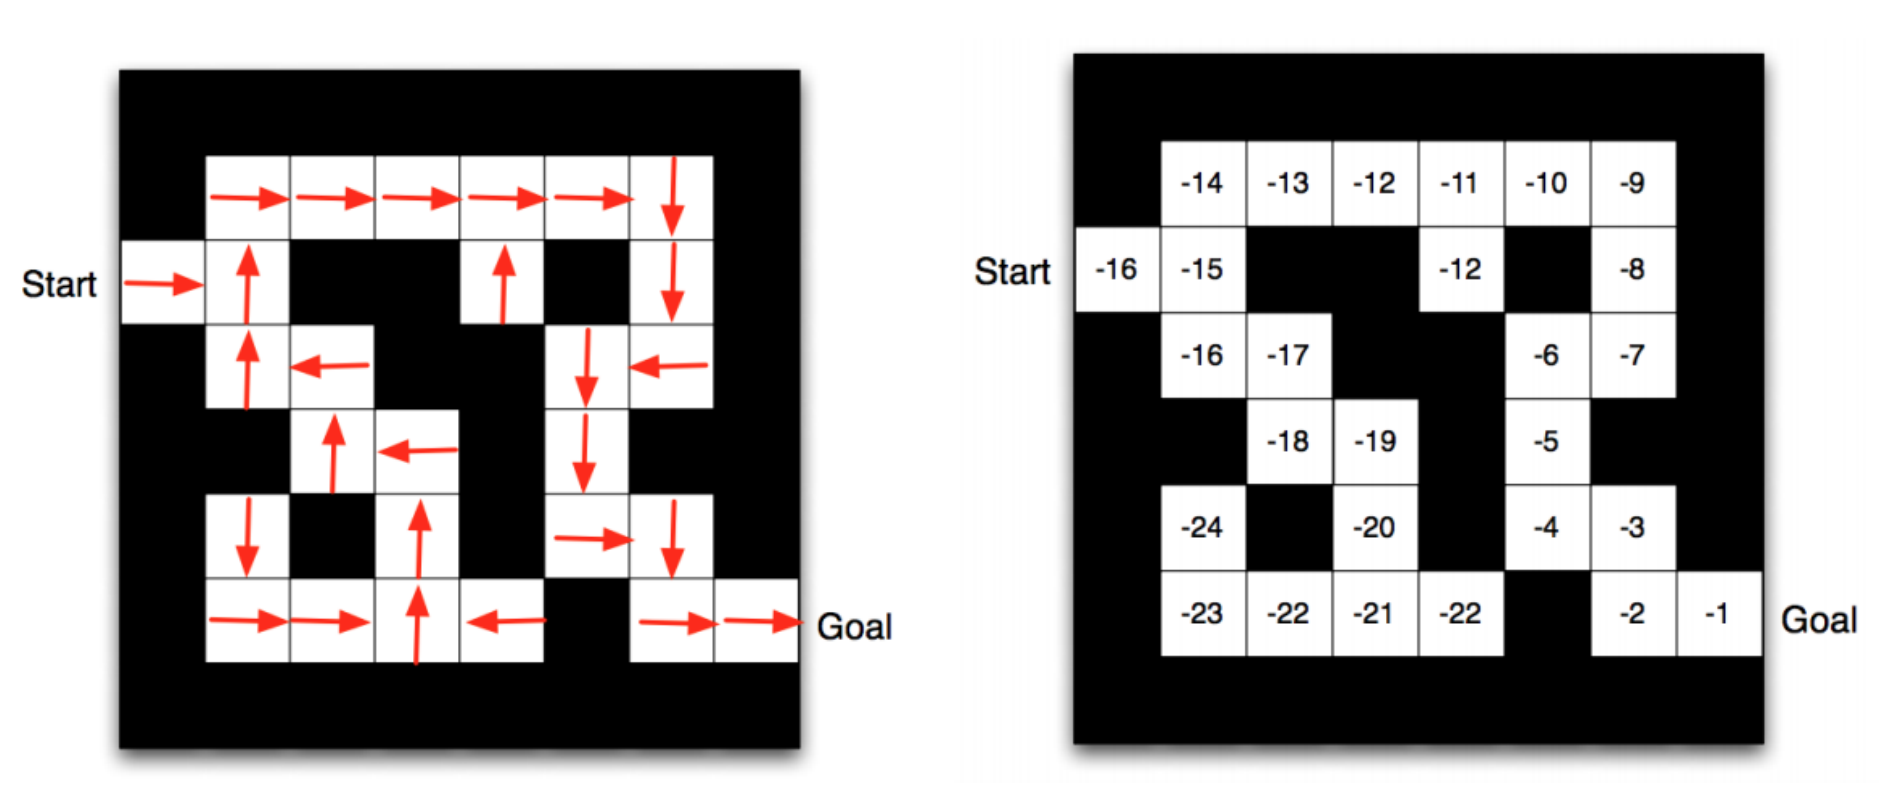
\includegraphics[width=0.9\textwidth,height=0.9\textheight,keepaspectratio]{images/intro/value.png}
\end{figure}

\end{frame}

\section{Q-Value Function}
\begin{frame}{Q-Value Function}
\begin{itemize}
    \item Can we use a value function to choose actions?
    $$\arg \max_a r(s_t,a) + \gamma \mathbb{E}_{p(s_{t+1}|s_t, a_t)}\left [ v^{\pi}(s_{t+1}) \right ]$$
    \pause
    \item \textbf{Problem:} this requires taking the expectation with respect to the environment’s dynamics, which we don’t have direct access to!
    \item Instead, learn a Q-value function.

\end{itemize}
\end{frame}

\begin{frame}{Q-Value Function}
\begin{itemize}
    \item The Q-value function at state s and action a, is the expected cumulative reward from taking action a in state s and then following the policy:
    $$Q^{\pi}(s,a) = \mathbb{E} \left [ \sum_{t \geq 0} \gamma^t r_t | s_0=0, a_0=a, \pi \right ]$$
    \item Relationship: $$V^{\pi}(s) = \sum_a \pi(a|s) Q^{\pi}(s,a)$$
    \item Optimal Action: $$\arg \max_a Q^{\pi}(s,a)$$
\end{itemize}
    
\end{frame}

\section{Bellman Equation}
\begin{frame}{Bellman Equation}
\begin{itemize}
    \item The Bellman Equation is a recursive formula for the Q-value function:
$$Q^{\pi}(s,a) =  r(s,a) + \gamma \mathbb{E}_{p(s'|s, a)\pi(a'|s')}\left [ Q^{\pi}(s',a') \right ]$$
    \item There are various Bellman equations, and most RL algorithms are
based on repeatedly applying one of them.
    
\end{itemize}

\item \textbf{Bellman Equations:}
\begin{itemize}
    \item For the value function $V^{\pi}(s)$:
    $$
    V^{\pi}(s) = \sum_{a} \pi(a|s) \sum_{s'} P(s'|s,a) \left[ R(s,a,s') + \gamma V^{\pi}(s') \right]
    $$
    \item For the Q-value function $Q^{\pi}(s,a)$:
    $$
    Q^{\pi}(s,a) = \sum_{s'} P(s'|s,a) \left[ R(s,a,s') + \gamma \sum_{a'} \pi(a'|s') Q^{\pi}(s',a') \right]
    $$
\end{itemize}
    
\end{frame}

\subsection{Optimal Bellman Equation}
\begin{frame}{Optimal Bellman Equation}
\begin{itemize}
    \item The optimal policy $\pi^{\star}$ is the one that maximizes the expected discounted reward, and the optimal Q-value function $Q^{\star}$ is the Q-value function for $\pi^{\star}$
    \item The Optimal Bellman Equation gives a recursive formula for $Q^{\star}$:
    $$Q^{\pi}(s,a) =  r(s,a) + \gamma \mathbb{E}_{p(s'|s, a)}\left [\max_{a'} Q^{\pi}(s_{t+1},a') | s_t=s, a_t=a \right ]$$
    \item This system of equations characterizes the optimal Q-value function. So maybe we can approximate $Q^{\star}$  by trying to solve the optimal Bellman equation!
    \item \textbf{Intuition}: If the optimal state-action values for the next time-step Q*(s’,a’) are known, then the optimal strategy is to take the action that maximizes the expected value of $r(s,a) + \gamma Q^{\pi}(s',a')$
    
\end{itemize}
    
\end{frame}